%Advanced Signal Processing mini project

% Titel: Principal Component Analysis used for evaluating separability of features extracted from raw EMG signal

\chapter*{Principal Component Analysis used for evaluating separability of features extracted from raw EMG signal.}

\section*{Description of problem}
Electromyography (EMG) is widely used as control input for functional prosthetics. Using classification as control scheme has shown a low error rate when testing hand movements in a clinical environment in a single limb position. However, a challenge occurs when changing limb position as the EMG alters when performing the same hand movements in a different limb position. A newer control scheme used is linear regression, which has shown robust proportional and simultaneous control in a single limb position. We will investigate if a linear regression-based control scheme can yield similar performance across limb positions. 
The raw EMG signal itself is not used as control input, but features extracted from it. In this study the commonly used Mean Absolute Value (MAV) feature, and the Logarithmic Variance (LogVar) feature, which has shown linear properties in studies, will be tested as control input for four different movements (extension, flexion, ulnar deviation and radial deviation). Before the linear regression models are build, it needs to be evaluated if the features extracted from the EMG signal (eight channel EMG) for each movement are separated enough for the models to distinguish between each movement. 

\begin{figure}[H] 
	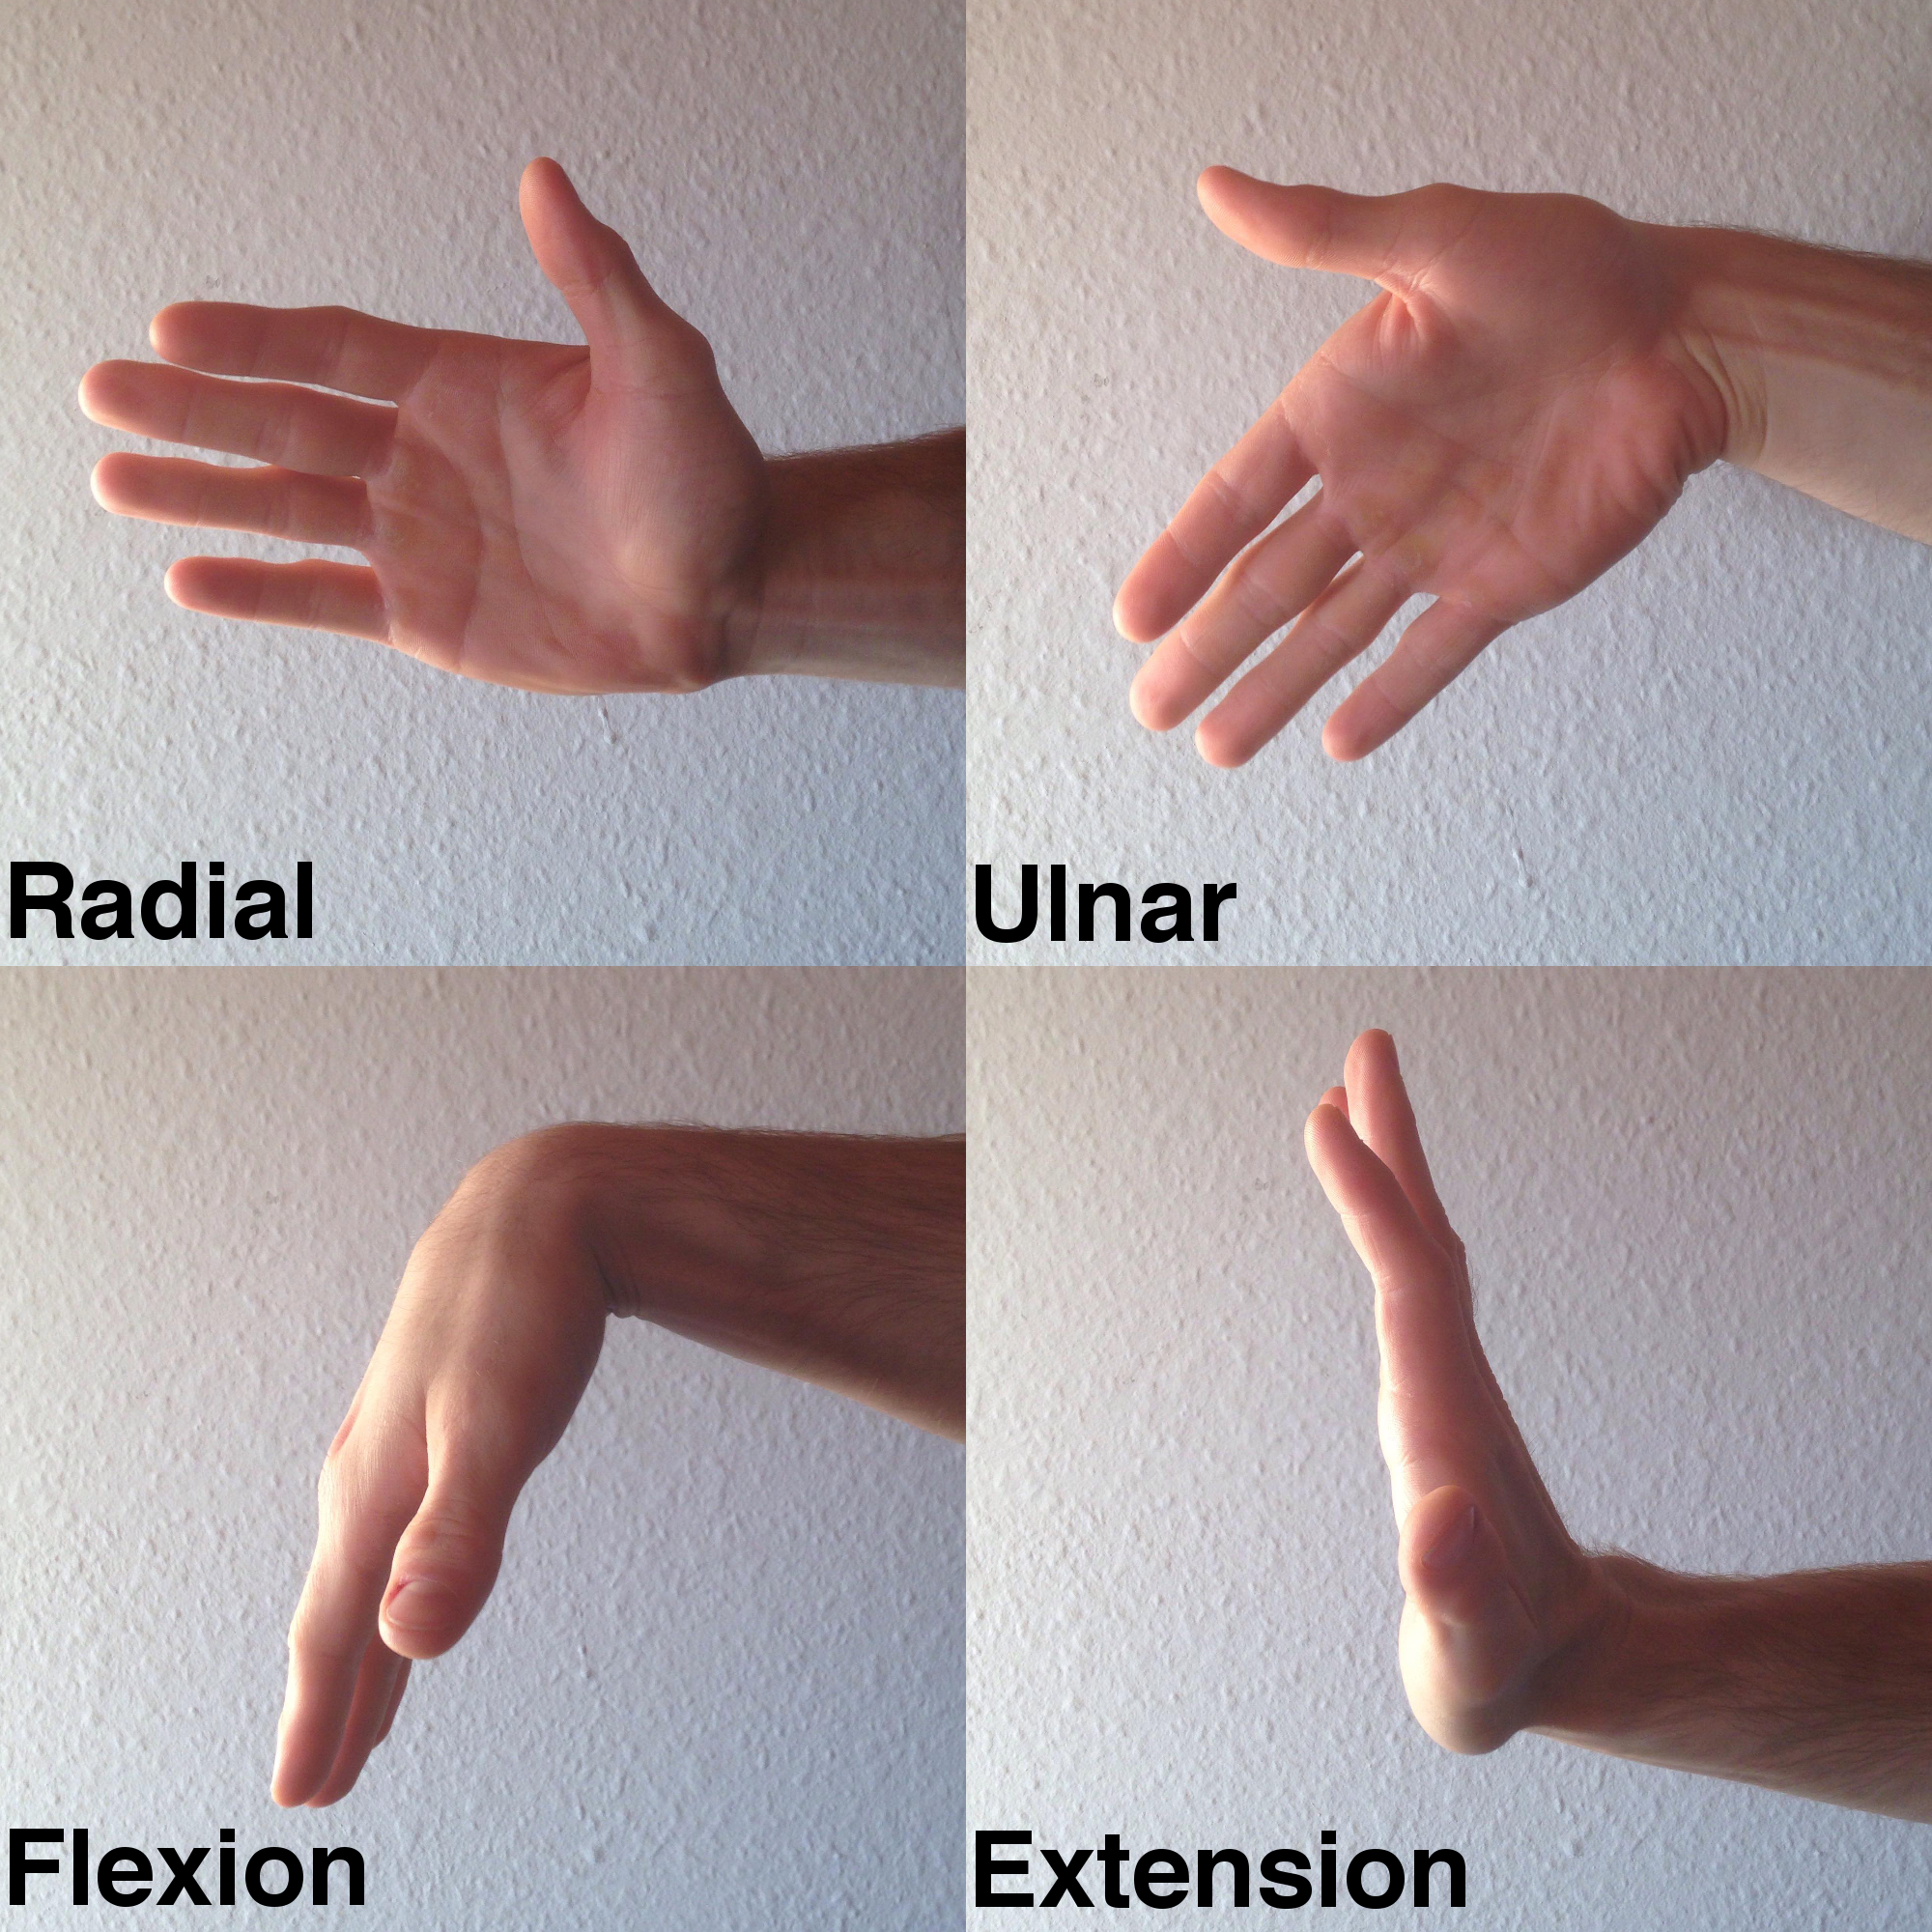
\includegraphics[width=0.3\textwidth]{figures/zASP/wristmovement}
	\caption{Hand gestures used when recording EMG signals.}
	\label{projection}
\end{figure}

\section*{Method of choice}
To solve this problem we choose to implement Principal Component Analysis (PCA). PCA is an analysis tool, used to find the most defining variables in a dataset. In this case by reducing an eight dimensional feature space to a three dimensional. Thus, being able to visualize the data and quantitatively evaluate the separability of the movements.

PCA is used to express a set of possible correlated variables into uncorrelated components, called principal components. A dataset of many variables can thus be expressed in a reduced dimensionality hyperspace using less variables that are the most defining for the given dataset. Each principal component (PC) is orthogonal on the former and are uncorrelated and have zero covariance. They each define the largest variance in an axis, such that PC 1 describes the direction of the maximum variance of the dataset. Each following PC describes the next highest variance of the dataset, with the constraint that is orthogonal and has zero covariance with any of the former PCs.
PCA is the orthogonal projection of data onto a lower dimension linear space. A PC is found by minimizing the variance by projecting the feature values (red dots) onto the line describing the highest variance in the data set (purple line) as seen on \figref{projection}. The PC (purple line) is found by minimizing the mean square distance between the data points. 

\begin{figure}[H] 
	\includegraphics[width=0.3\textwidth]{figures/zASP/projection}
	\caption{Projection of data variables (red dots) onto principal component line (purple)}
	\label{projection}
\end{figure}

The algebraic method of calculating the PCs is by using Singular Value Decomposition (SVD). The first step is to compute the squared cross product matrix of variances and covariances among every pair of the variables in the data set, where the diagonals are the variances and the off-diagonals are the covariances, as done in the following equation:

\begin{equation}
S = X \textquoteright X
\end{equation}
Where S is the cross product and X is the dataset matrix. When finding the PCs it includes an eigen-analysis of S. The eigenvalues of are solutions to the following equation:
%\verticalspace{1}
\begin{equation}
| S - \lambda |  = 0
\end{equation}

Where $\lambda$ is the variances of each PC and I is the identity matrix. After solving for $\lambda$ the eigenvectors can be solved through the following equation:

\begin{equation}
det | S - \lambda | b_{i} = 0
\end{equation}
Where $b_{i}$ is used to calculate the eigenvectors as in:

\begin{eqnarray}
u_{i} = \frac{b_{i}}{\sqrt{b_{i}^{\textquoteright} b_{i}}}
\end{eqnarray}

Where $u_{i}$ is the i number of eigenvectors that contain a contribution to the principal components.
The SVD orders the eigenvalues by size $\lambda_{1} > \lambda_{2} … > \lambda_{M}$. The scores for each PC is equal to the corresponding eigenvalue for that exact axis. The eigenvalues describe how much of the variance is accounted for by the associated PC. Summation of all eigenvalues accounts for the total variance of the data set; this is called the trace. To find how much the each PC accounts for, the eigenvalue of that PC is divided by the total variance: $\%~ of~ total~ variance~ = \frac{PC}{Trace}$. This can be used for deciding how many components are significant and by how much the dataset can be reduced. In our case this choice is made, due to the intention of visualizing the PC’s in a three dimensional space. 
MatLab code for implementation is shown in the appendix after the results.

\section*{Results}

When applying PCA on the MAV features for the four movements it is seen that three components describe 93.8 \% of the data set. Plotting the three first PCs for each movement illustrates a separability between the movements, see \figref{PCAMAV}. Thus, the MAV feature extracted from the acquired data can be used to build linear regression models that distinguish between the four movements. The same separability is found for the LogVar feature, see \figref{PCALogVar}, where the first three PCs accounts for 93.97 \% of the total variance. 

\begin{figure}[H] 
	\includegraphics[width=0.9\textwidth]{figures/zASP/pcasubplotMAV}
	\caption{PCA of MAV features}
	\label{PCAMAV}
\end{figure}

\begin{figure}[H] 
	\includegraphics[width=0.9\textwidth]{figures/zASP/pcasubplotLogVar}
	\caption{PCA of LogVar features}
	\label{PCALogVar}
\end{figure}



\section*{Appendix: MatLab implementation}

\lstinputlisting{contents/zxzASPminiProject/goScatterPlot.m}

